% ============================================================
%  Příprava na maturitu – Elektrotechnika
%  Okruh 17: Optoelektronika
% ============================================================

\documentclass[a4paper,10pt]{article}

\usepackage[T1]{fontenc}
\usepackage[utf8]{inputenc}
\usepackage[left=2.0cm, right=1.8cm, top=1.8cm, bottom=1.8cm]{geometry}
\usepackage{parskip}
\usepackage{xcolor}
\usepackage{tabularx}
\usepackage{booktabs}
\usepackage{tikz}
\usepackage{mdframed}
\usepackage{amsmath}
\usepackage{enumitem}
\usepackage{circuitikz}

\usetikzlibrary{arrows.meta, positioning, decorations.pathmorphing, shapes.geometric, calc}

% --- Barvy ---
\definecolor{accent}{HTML}{1A3A5C}
\definecolor{lightblue}{HTML}{EAF2F8}
\definecolor{lightyellow}{HTML}{FDFBE4}
\definecolor{lightgreen}{HTML}{EAF7EA}
\definecolor{lightred}{HTML}{FDE8E8}
\definecolor{lightgray}{HTML}{F4F4F4}

% --- Boxy ---
\newmdenv[backgroundcolor=lightblue,linecolor=accent!40,roundcorner=4pt,
  innertopmargin=6pt,innerbottommargin=6pt,innerleftmargin=8pt,innerrightmargin=8pt]{pojmybox}
\newmdenv[backgroundcolor=lightyellow,linecolor=accent!30,roundcorner=4pt,
  innertopmargin=6pt,innerbottommargin=6pt,innerleftmargin=8pt,innerrightmargin=8pt]{vysvetlenibox}
\newmdenv[backgroundcolor=lightgreen,linecolor=accent!40,roundcorner=4pt,
  innertopmargin=6pt,innerbottommargin=6pt,innerleftmargin=8pt,innerrightmargin=8pt]{vzorcebox}
\newmdenv[backgroundcolor=lightred,linecolor=accent!30,roundcorner=4pt,
  innertopmargin=6pt,innerbottommargin=6pt,innerleftmargin=8pt,innerrightmargin=8pt]{durazbox}

\setlist[itemize]{noitemsep, leftmargin=1.4em, topsep=2pt}
\setlist[enumerate]{noitemsep, leftmargin=1.4em, topsep=2pt}

% --- Zkratka pro jednotky ---
\newcommand{\jednotka}[1]{\,[\mathrm{#1}]}

\begin{document}

% ============================================================
\section*{\large Okruh 17 – Optoelektronika}

\begin{pojmybox}
\textbf{Klíčové pojmy:}
elektromagnetické záření, spektrum, foton, luminiscence, fotoelektrický jev, LED, laserová dioda (LD), fotorezistor, fotodioda, fototranzistor, optočlen (galvanické oddělení), optické vlákno, index lomu, totální odraz
\end{pojmybox}

\begin{vysvetlenibox}

% ================================================================
\subsection*{1. Světlo jako elektromagnetické vlnění}

Optoelektronika propojuje elektrické a optické jevy. Pracuje s elektromagnetickým zářením v oblastech:
\begin{itemize}
    \item \textbf{Ultrafialové (UV):} vlnové délky menší než $380\,\mathrm{nm}$.
    \item \textbf{Viditelné světlo (VIS):} vlnové délky $380\,\mathrm{nm}$ (fialová) až $780\,\mathrm{nm}$ (červená).
    \item \textbf{Infračervené (IR):} vlnové délky větší než $780\,\mathrm{nm}$ (typicky dálkové ovladače, noční vidění).
\end{itemize}

Světlo můžeme chápat i jako proud částic – \textbf{fotonů}. Energie jednoho fotonu roste s rostoucí frekvencí (kratší vlnovou délkou).

\begin{vzorcebox}
\[
E = h \cdot f = h \cdot \frac{c}{\lambda} \jednotka{J}
\]
kde $E$ = energie fotonu, $h$ = Planckova konstanta, $f$ = frekvence [Hz], $c$ = rychlost světla ve vakuu ($3\cdot 10^8\,\mathrm{m/s}$), $\lambda$ = vlnová délka [m].
\end{vzorcebox}

% ================================================================
\subsection*{2. Zdroje optického záření (Elektřina $\to$ Světlo)}

Využívají jev \textbf{elektroluminiscence} – při průchodu elektrického proudu polovodičovým PN přechodem v propustném směru dochází k rekombinaci elektronů s děrami, přičemž se přebytečná energie vyzáří ve formě fotonu.

\begin{itemize}
    \item \textbf{Svítivá dioda (LED):} Vydává neuspořádané (nekoherentní) světlo určité vlnové délky (barvy). Barva světla (energie fotonu) závisí výhradně na použitém materiálu polovodiče. 
    \item \textbf{Laserová dioda (LD):} Světlo vzniká tzv. stimulovanou emisí. Vyzařuje \textbf{koherentní} světlo (všechny fotony mají stejnou fázi, vlnovou délku a směr). Paprsek se nerozptyluje. Použití: Čtečky čárových kódů, optické mechaniky, optické sítě.
\end{itemize}

% ================================================================
\subsection*{3. Detektory záření (Světlo $\to$ Elektřina)}

Využívají \textbf{vnitřní fotoelektrický jev}. Foton dopadne do polovodiče, předá svou energii elektronu, vytrhne ho z atomového obalu (vznikne volný elektron a díra) a tím se zvýší vodivost materiálu.

\begin{center}
\begin{tabularx}{0.97\linewidth}{@{} l X @{}}
\toprule
\textbf{Typ detektoru} & \textbf{Princip a vlastnosti} \\
\midrule
\textbf{Fotorezistor (LDR)} & Kus polovodiče (bez PN přechodu). S rostoucím osvětlením jeho odpor **klesá** (z $\mathrm{M\Omega}$ ve tmě na stovky $\Omega$ na slunci). Je velmi **pomalý**. Použití: Soumrakové spínače. \\
\textbf{Fotodioda} & Obsahuje PN přechod. Zapojuje se v **závěrném směru**. Světlo generuje volné náboje $\implies$ vzniká proud přímo úměrný osvětlení. Je extrémně **rychlá** (MHz až GHz). Použití: Přijímače v optických sítích, IR dálkové ovladače. \\
\textbf{Fototranzistor} & Funguje jako fotodioda integrovaná do báze tranzistoru. Proud generovaný světlem je rovnou zesílen (činitel $\beta$). Je mnohem **citlivější**, ale pomalejší než samotná fotodioda. \\
\textbf{Fotovoltaický článek} & Fotodioda s ohromnou plochou, ze které se odebírá výkon. Generuje napětí (cca 0,6 V). (\textit{Navazuje na Okruh 8: Výroba energie}). \\
\bottomrule
\end{tabularx}
\end{center}

% ================================================================
\subsection*{4. Optočleny (Galvanické oddělení)}

Optočlen (optokoupler) je součástka, která v jednom neprůhledném pouzdře spojuje zdroj záření (LED) a detektor (fototranzistor).

\textbf{K čemu slouží?} 
K dokonalému \textbf{galvanickému oddělení} dvou částí obvodu. Signál se přenáší pouze světlem, neexistuje žádné vodivé spojení. Používá se k ochraně citlivých číslicových obvodů (např. mikrokontroléru) před vysokým napětím a rušením (např. řízení 230V motorů nebo přenos dat ze spínaného zdroje). Izolační bariéra běžně vydrží i $5000\,\mathrm{V}$.

\begin{center}
\begin{circuitikz}[font=\small, thick]
  % Hranice optočlenu
  \draw[fill=lightgray!20, dashed, draw=gray] (-0.5, -0.5) rectangle (3.5, 3);
  \node[above, font=\bfseries] at (1.5, 3) {Pouzdro optočlenu};
  \draw[dashed, blue!50, line width=1.5pt] (1.5, -0.5) -- (1.5, 3) node[midway, sloped, above, text=black] {Galvanická bariéra};

  % Vstupní část (LED)
  \draw (-2.5, 2.5) node[left] {IN (Signál)} to[R, l=$R_{in}$, o-] (-0.5, 2.5) 
        -- (0.5, 2.5) to[leD] (0.5, 0.5) -- (-0.5, 0.5) 
        to[short, -o] (-2.5, 0.5) node[left] {GND1 (Zem PC)};

  % Výstupní část (Fototranzistor NPN)
  \draw (2.5, 1.5) node[npn, photo, anchor=B] (ptr) {};
  \draw (ptr.C) -- (2.5, 2.5) to[short, -o] (4.5, 2.5) node[right] {+5V ($V_{CC}$)};
  \draw (ptr.E) -- (2.5, 0.5) to[short, -o] (4.5, 0.5) node[right] {GND2 (Zem modulu)};
  
  % Výstup s Pull-down rezistorem
  \draw (2.5, 1.5) ++(0.5, -0.5) to[short, *-o] (4.5, 1) node[right] {OUT (Řízení)};
  \draw (3.5, 1) to[R, l=$R_L$, *-*] (3.5, 0.5);

\end{circuitikz}
\end{center}

% ================================================================
\subsection*{5. Optická vlákna a komunikace}

Optická vlákna nahrazují metalické (měděné) kabely v telekomunikacích. Skládají se ze skleněného \textbf{jádra} a skleněného \textbf{pláště}, které jsou chráněny kevlarovou ochranou a vnějším obalem.

\textbf{Fyzikální princip (Totální odraz):}\\
Jádro má mírně \textbf{větší index lomu} než plášť ($n_1 > n_2$). Pokud světlo vstupuje do jádra pod správným úhlem, nedokáže proniknout do pláště (světlo se láme od kolmice). Jakmile úhel překročí tzv. mezní úhel, dojde k \textbf{úplnému (totálnímu) odrazu} a světlo se odráží od rozhraní zpět do jádra. Vlákno funguje jako dokonalé zrcadlové potrubí.

\begin{center}
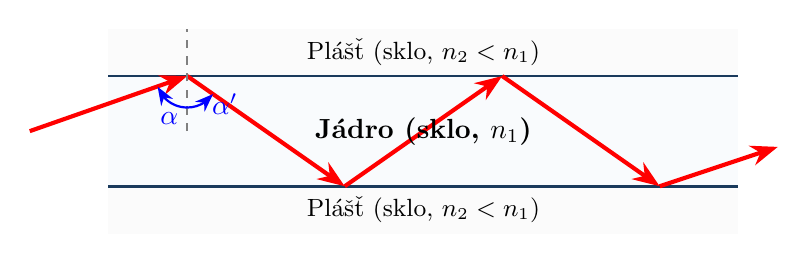
\begin{tikzpicture}[>=Stealth, thick]
  % Jádro
  \draw[fill=lightblue!30, draw=none] (0, 0.8) rectangle (8, 2.2);
  % Plášť (horní a dolní)
  \draw[fill=lightgray!40, draw=none] (0, 2.2) rectangle (8, 2.8);
  \draw[fill=lightgray!40, draw=none] (0, 0.2) rectangle (8, 0.8);
  
  % Rozhraní (linky)
  \draw[line width=1pt, accent] (0, 2.2) -- (8, 2.2);
  \draw[line width=1pt, accent] (0, 0.8) -- (8, 0.8);
  
  % Paprsek světla
  \draw[red, line width=1.5pt, ->] (-1, 1.5) -- (1, 2.2);
  \draw[red, line width=1.5pt, ->] (1, 2.2) -- (3, 0.8);
  \draw[red, line width=1.5pt, ->] (3, 0.8) -- (5, 2.2);
  \draw[red, line width=1.5pt, ->] (5, 2.2) -- (7, 0.8);
  \draw[red, line width=1.5pt, ->] (7, 0.8) -- (8.5, 1.3);

  % Kolmice a úhly na prvním odrazu
  \draw[dashed, gray] (1, 1.5) -- (1, 2.8);
  \draw[blue, ->] (1, 1.8) arc (-90:-160:0.4) node[midway, below] {$\alpha$};
  \draw[blue, ->] (1, 1.8) arc (-90:-35:0.4) node[midway, right] {$\alpha'$};

  % Popisky vrstev
  \node[font=\bfseries] at (4, 1.5) {Jádro (sklo, $n_1$)};
  \node[font=\small] at (4, 2.5) {Plášť (sklo, $n_2 < n_1$)};
  \node[font=\small] at (4, 0.5) {Plášť (sklo, $n_2 < n_1$)};
\end{tikzpicture}
\end{center}

\begin{durazbox}
\textbf{Dělení optických vláken:}
\begin{itemize}
    \item \textbf{Mnohovidová (Multimode - MM):} Jádro je tlustší ($50\,\mathrm{\mu m}$). Paprsky (vidy) se odrážejí pod různými úhly, čímž vzniká disperze (rozmazání pulzů). Použití: Krátké vzdálenosti (stovky metrů, LAN sítě). Zdroj: Levná LED nebo VCSEL.
    \item \textbf{Jednovidová (Singlemode - SM):} Jádro je extrémně tenké ($9\,\mathrm{\mu m}$). Světlo se nešíří odrazem, ale letí přímo středem (pouze jeden vid). Žádná disperze. Použití: Dlouhé trasy (stovky kilometrů, podmořské kabely). Zdroj: Laser.
\end{itemize}
\end{durazbox}

\textbf{Výhody optických sítí (oproti měděným kabelům):}
Ohromná přenosová rychlost (běžně v řádech Terabitů/s), imunita proti vnějšímu elektromagnetickému rušení (vedle kabelu může uhodit blesk a signál to neovlivní), bezpečnost proti odposlechu, nízká hmotnost a dlouhá životnost.

\end{vysvetlenibox}

\end{document}